\documentclass[12pt, a4paper]{article}

% ==========================================
% 1. KHAI BÁO GÓI THƯ VIỆN (PACKAGES)
% ==========================================
% Bảng mã & Font chữ
\usepackage[utf8]{inputenc}
\usepackage[T5]{fontenc}

% Toán học
\usepackage{amsmath, amssymb}

% Căn lề & Bố cục trang
\usepackage[top=2.2cm, bottom=1.5cm, left=1cm, right=1cm, headheight=15pt]{geometry}
\usepackage{fancyhdr}
\usepackage{needspace}
\usepackage{tkz-tab}

% Đồ họa & Màu sắc
\usepackage{xcolor}
\usepackage{graphicx} 
\usepackage{tikz}
\usetikzlibrary{calc, shapes.geometric, positioning}


% Bảng biểu & Danh sách
\usepackage{colortbl}
\usepackage{array}
\usepackage{makecell}
\usepackage{multirow}
\usepackage{tasks}

% Biểu tượng
\usepackage{fontawesome5}

% ==========================================
% 2. THIẾT LẬP MÀU SẮC CHỦ ĐẠO
% ==========================================
\definecolor{goldyellow}{RGB}{255, 179, 0}
\definecolor{amberorange}{RGB}{230, 115, 0}
\definecolor{lightamber}{RGB}{255, 248, 225}
\definecolor{deepblue}{RGB}{25, 42, 86}
\definecolor{accentred}{RGB}{232, 65, 24}
\definecolor{softgray}{RGB}{220, 220, 222} 
\definecolor{fbblue}{RGB}{15, 80, 200}


% ==========================================
% 3. CẤU HÌNH HEADER & FOOTER
% ==========================================
\pagestyle{fancy}
\fancyhf{}
\renewcommand{\headrulewidth}{0pt}

% Khai báo biến lưu trữ nội dung góc phải của Header
\newcommand{\HeaderRightText}{}

% --- Header ---
\fancyhead[C]{
    \begin{tikzpicture}[remember picture, overlay]
        
        % Dải màu trang trí góc trên
        \path[fill=deepblue] (current page.north west) -- (current page.north east) 
            -- ($(current page.north east) + (0, -1.6cm)$) 
            .. controls ($(current page.north) + (3, -2.0cm)$) and ($(current page.north) + (-3, -0.4cm)$) .. 
            ($(current page.north west) + (0, -1.0cm)$) -- cycle;
            
        \path[fill=goldyellow] (current page.north west) -- (current page.north east) 
            -- ($(current page.north east) + (0, -1.0cm)$) 
            .. controls ($(current page.north) + (4, -1.0cm)$) and ($(current page.north) + (-2, -2.2cm)$) .. 
            ($(current page.north west) + (0, -1.6cm)$) -- cycle;
            
        \path[fill=amberorange] (current page.north west) -- ($(current page.north west) + (6.5cm, 0)$) 
            .. controls ($(current page.north west) + (4.5cm, -1.2cm)$) and ($(current page.north west) + (2cm, -2.0cm)$) .. 
            ($(current page.north west) + (0, -2.0cm)$) -- cycle;
            
        % Logo góc trái Header
        \node[anchor=west, inner sep=0pt] 
            at ($(current page.north west) + (0cm, -0.8cm)$) {
\includegraphics[height=2.0cm]{../../../image/logo-header.png}};
            
        % Text góc phải Header (Tự động lấy từ đối số thứ 3 của \titlebox)
        \node[anchor=east, text=white, font=\small\bfseries\sffamily] 
            at ($(current page.north east) + (-0.8cm, -0.5cm)$) {\HeaderRightText};
    \end{tikzpicture}
}

% --- Footer ---
\fancyfoot[C]{
    \begin{tikzpicture}[remember picture, overlay]
        % Đường kẻ ngang
        \draw[amberorange, line width=1.5pt] 
            ($(current page.south west) + (0cm, 0.4cm)$) -- ($(current page.south east) + (0cm, 0.4cm)$);

        % Dải cong góc phải
        \path[fill=goldyellow] (current page.south east) -- ($(current page.south east) + (-5cm, 0)$) 
            .. controls ($(current page.south east) + (-3cm, 0.8cm)$) and ($(current page.south east) + (-1.5cm, 1.2cm)$) .. 
            ($(current page.south east) + (0, 1.2cm)$) -- cycle;

        % Mạng xã hội
        \node[anchor=west, inner sep=0pt] at ($(current page.south west) + (1cm, 0.8cm)$) {
            \small\sffamily
            \textcolor{fbblue}{\faFacebook\hskip 4pt Toán Anh Huy MATH-STER}
            \hskip 18pt
            \textcolor{black}{\faTiktok\hskip 4pt huymathster}
        };

        % Số trang (Thiết kế hình tròn cũ thu nhỏ)
        \node[circle, fill=white, draw=amberorange, line width=1.5pt, text=deepblue, font=\large\bfseries, inner sep=0pt, minimum size=0.7cm] 
            at ($(current page.south east) + (-1.0cm, 0.65cm)$) {\thepage};
    \end{tikzpicture}
}

% ==========================================
% 4. ĐỊNH NGHĨA MACRO: KHUNG TIÊU ĐỀ
% ==========================================
\newcommand{\titlebox}[3]{
    % Gán nội dung đối số #3 vào biến HeaderRightText
    \gdef\HeaderRightText{#3}
    
    \begin{center}
    \vspace*{-0.5cm}
    \begin{tikzpicture}
        % Khung vô hình (Phantom Box) định chuẩn kích thước
        \node[text width=16cm, inner xsep=0pt, inner ysep=16pt, opacity=0] (MainBox) {
            \begin{minipage}[c]{4.2cm}
                \centering\vspace{0.1cm}
                \rule{2.2cm}{2.2cm} 
                \vspace{0.1cm}
            \end{minipage}%
            \begin{minipage}[c]{11.5cm}
                \centering\vspace{0.15cm}
                {\huge\bfseries\sffamily #2 \par}
                \vspace{0.15cm} 
            \end{minipage}
        };
        
        % Đổ bóng & Nền
        \fill[goldyellow, rounded corners=8pt] ([xshift=5pt, yshift=-5pt]MainBox.south west) rectangle ([xshift=5pt, yshift=-5pt]MainBox.north east);
        \fill[white, rounded corners=8pt] (MainBox.south west) rectangle (MainBox.north east);
        
        % Lưới ô ly & Nền Logo
        \begin{scope}
            \clip[rounded corners=8pt] (MainBox.south west) rectangle (MainBox.north east);
            \draw[step=0.4cm, softgray!50, line width=0.6pt] (MainBox.south west) grid (MainBox.north east);
            \fill[lightamber!60] (MainBox.south west) rectangle ([xshift=4.2cm]MainBox.north west);
        \end{scope}

        % Viền ngoài
        \draw[deepblue, line width=1.5pt, rounded corners=8pt] (MainBox.south west) rectangle (MainBox.north east);

        % Nội dung Text (Lớp trên cùng)
        \node[text width=16cm, inner xsep=0pt, inner ysep=16pt] at (MainBox.center) {
            \begin{minipage}[c]{4.2cm}
                \centering
                % --- ĐIỀU CHỈNH TỌA ĐỘ LOGO Ở ĐÂY ---
                \hspace*{-0.5cm}\raisebox{-0.2cm}{
\includegraphics[width=5.5cm]{../../../image/logo.png}}
            \end{minipage}%
            \begin{minipage}[c]{11.5cm}
                \centering\vspace{0.15cm}
                {\huge\bfseries\sffamily\color{deepblue} #2 \par}
                \vspace{0.15cm} 
            \end{minipage}
        };
        
        % Trang trí phụ kiện
        \draw[deepblue, line width=1.5pt, dashed] ([xshift=4.2cm]MainBox.north west) -- ([xshift=4.2cm]MainBox.south west);
        \node[regular polygon, regular polygon sides=4, rotate=45, fill=white, draw=accentred, line width=1.2pt, inner sep=2.5pt] at ([xshift=4.2cm]MainBox.west) {};
        \node[anchor=west, fill=amberorange, text=white, font=\large\bfseries\sffamily, rounded corners=4pt, draw=deepblue, line width=1.5pt, inner xsep=12pt, inner ysep=6pt] at ([xshift=1.5cm]MainBox.north west) {#1};
        \fill[accentred] ([xshift=-1.8cm, yshift=-0.4cm]MainBox.north east) circle (3pt);
        \fill[amberorange] ([xshift=-1.4cm, yshift=-0.4cm]MainBox.north east) circle (3pt);
        \fill[goldyellow] ([xshift=-1.0cm, yshift=-0.4cm]MainBox.north east) circle (3pt);
    \end{tikzpicture}
    \vspace*{0cm}
    \end{center}
}

% ==========================================
% 5. ĐỊNH NGHĨA MACRO: CẤU TRÚC CÂU HỎI (ÉP SÁT NHAU)
% ==========================================
\newcommand{\questioncore}[2]{
    % Xóa khoảng cách phía trên, ép sát câu trước
    \noindent \textbf{\textcolor{deepblue}{Câu #1.} \textcolor{accentred}{[STER]}} #2
    \par\nopagebreak
}

% Cấu hình hiển thị đáp án trắc nghiệm
\settasks{
    label=\textbf{\textcolor{amberorange}{\Alph*.}}, 
    label-width=15pt,     
    item-indent=25pt,     
    label-offset=6pt,    
    column-sep=20pt,     
    after-item-skip=2pt  % Đã giảm tối đa khoảng cách giữa các dòng đáp án A B C D
}

% Hàm vẽ dòng kẻ nháp
\newcommand{\drawdashlines}[1]{
    \ifnum#1>0
        \nopagebreak\vspace{0.1cm}\noindent 
        \begin{tikzpicture}
            \foreach \i in {1,...,#1} {
                \draw[softgray, line width=0.2pt] (0,-{\i*0.7}) -- (\textwidth-4pt,-{\i*0.7});
            }
        \end{tikzpicture}
        \par
    \fi
    % Đã xóa hoàn toàn khoảng cách thừa ở nhánh else
}

% --- Dạng 1: Trắc nghiệm 4 đáp án ---
\newcommand{\questionLinesManual}[4]{
    \pgfmathsetmacro{\calculatedSpace}{1.5 + #1 * 0.65}
    \needspace{\calculatedSpace cm} 
    \questioncore{#2}{#3}
    #4
    \par\nopagebreak
    \drawdashlines{#1}
}

\usepackage{cellspace}
\setlength\cellspacetoplimit{4pt}    % Khoảng đệm tự động phía trên ô
\setlength\cellspacebottomlimit{4pt} % Khoảng đệm tự động phía dưới ô




\newcommand{\questionTrueFalse}[4]{
    \pgfmathsetmacro{\calculatedSpace}{3.0 + #1 * 0.65} 
    \needspace{\calculatedSpace cm}
    \questioncore{#2}{#3}
    
    \nopagebreak
    \begin{center}
    \begin{tabular}{|>{\centering\arraybackslash}S{m{0.8cm}}|S{m{12cm}}|>{\centering\arraybackslash}S{m{1.5cm}}|>{\centering\arraybackslash}S{m{1.5cm}}|}
        \hline
        \rowcolor{amberorange!20}
        \multicolumn{1}{|c|}{} & \multicolumn{1}{>{\centering\arraybackslash}m{12cm}|}{\textbf{\textcolor{deepblue}{Mệnh đề}}} & 
        \textbf{\textcolor{deepblue}{Đúng}} & 
        \textbf{\textcolor{deepblue}{Sai}} \\
        \hline
        #4
        \hline
    \end{tabular}
    \end{center}
    
    \par\nopagebreak
    \drawdashlines{#1}
}

% ----- Dạng 3: Tự luận ngắn -----
\newcommand{\questionShortAnswer}[3]{
    \pgfmathsetmacro{\calculatedSpace}{1.5 + #1 * 0.8}
    \needspace{\calculatedSpace cm}
    
    {\linespread{1.1}\selectfont % Bóp nhỏ giãn dòng của câu tự luận
    \questioncore{#2}{#3}\par}
    
    \nopagebreak
    \begin{flushright}
        \begin{tikzpicture}
            \node[anchor=east, font=\small\bfseries\sffamily, text=deepblue] 
                at (-0.2, 0.4) {Đáp án:};
            \fill[goldyellow, rounded corners=3pt] (0.08, -0.08) rectangle (3.08, 0.72);
            \draw[draw=deepblue, fill=white, line width=1.2pt, rounded corners=3pt] 
                (0,0) rectangle (3.0, 0.8);
            \foreach \x in {0.75, 1.5, 2.25} {
                \draw[draw=deepblue, line width=0.6pt] (\x, 0) -- (\x, 0.8);
            }
        \end{tikzpicture}
    \end{flushright}
    
    \par\nopagebreak
    \drawdashlines{#1}
}


\settasks{
    after-item-skip = 1em % Tương đương row-skip cũ
}

% ==========================================
% BẮT ĐẦU NỘI DUNG TÀI LIỆU
% ==========================================
\begin{document}

% Truyền 3 tham số: {Nhãn cam} {Chữ to chính giữa} {Chữ ở góc phải Header}
\titlebox{Chủ đề: Tích phân}{Ứng dung tích phân tính diện tích thể tính}{Nguyên hàm - Tích phân: Ứng dụng}

% --- CÂU 1 ---
\questionLinesManual{10}{1}{Cho hàm số \( y = f(x) \) xác định và liên tục trên đoạn \([a; b]\). Diện tích hình phẳng giới hạn bởi đồ thị hàm số \( y = f(x) \), trục hoành và hai đường thẳng \( x = a, \, x = b \) được tính theo công thức}{%
    \begin{tasks}(4)
        \task \( S = \displaystyle\int_a^b |f(x)| dx \)
        \task \( S = \displaystyle\int_a^b f(x) dx \)
        \task \( S = -\displaystyle\int_a^b f(x) dx \)
        \task \( S = \displaystyle\int_a^b |f(x)| dx \)
    \end{tasks}
}

% --- CÂU 2 ---
\questionLinesManual{10}{2}{Diện tích \( S \) của hình phẳng giới hạn bởi các đường \( y = 2x^2 \), \( y = -1 \), \( x = 0 \) và \( x = 1 \) được tính bởi công thức nào sau đây?}{%
    \begin{tasks}(4)
        \task \( \displaystyle S = \pi \int_{0}^{1} (2x^2 + 1) dx \)
        \task \( \displaystyle S = \int_{0}^{1} (2x^2 - 1) dx \)
        \task \( \displaystyle S = \int_{0}^{1} (2x^2 + 1)^2 dx \)
        \task \( \displaystyle S = \int_{0}^{1} (2x^2 + 1) dx \)
    \end{tasks}
}

% --- CÂU 3 ---
\questionLinesManual{10}{3}{Diện tích hình phẳng giới hạn bởi hai đường \( y = x^2 - 4 \) và \( y = 2x - 4 \) bằng}{%
    \begin{tasks}(4)
        \task 36
        \task \( \dfrac{4}{3} \)
        \task \( \dfrac{4\pi}{3} \)
        \task \( 36\pi \)
    \end{tasks}
}

% --- CÂU 4 ---
\questionLinesManual{10}{4}{Diện tích hình phẳng giới hạn bởi hai đường \( y = x^2 - 1 \) và \( y = x - 1 \) bằng}{%
    \begin{tasks}(4)
        \task \( \dfrac{\pi}{6} \)
        \task \( \dfrac{13}{6} \)
        \task \( \dfrac{13\pi}{6} \)
        \task \( \dfrac{1}{6} \)
    \end{tasks}
}

% --- CÂU 5 ---
\questionLinesManual{10}{5}{Diện tích hình phẳng giới hạn bởi hai đường \( y = x^2 - 3 \) và \( y = x - 3 \) bằng}{%
    \begin{tasks}(4)
        \task \( \dfrac{125\pi}{6} \)
        \task \( \dfrac{1}{6} \)
        \task \( \dfrac{125}{6} \)
        \task \( \dfrac{\pi}{6} \)
    \end{tasks}
}

% --- CÂU 6 ---
\questionLinesManual{10}{6}{Gọi \( S \) là diện tích của hình phẳng giới hạn bởi các đường \( y = 2^x \), \( y = 0 \), \( x = 0 \), \( x = 2 \). Mệnh đề nào dưới đây đúng?}{%
    \begin{tasks}(4)
        \task \( \displaystyle S = \int_{0}^{2} 2^x dx \)
        \task \( \displaystyle S = \int_{0}^{2} 2^x dx \)
        \task \( \displaystyle S = \pi \int_{0}^{2} 2^x dx \)
        \task \( \displaystyle S = \int_{0}^{2} 2^{2x} dx \)
    \end{tasks}
}

% --- CÂU 7 ---
\questionLinesManual{10}{7}{Gọi \( S \) là diện tích hình phẳng giới hạn bởi các đường \( y = e^x \), \( y = 0 \), \( x = 0 \), \( x = 2 \). Mệnh đề nào dưới đây đúng?}{%
    \begin{tasks}(4)
        \task \( \displaystyle S = \int_{0}^{2} e^x dx \)
        \task \( \displaystyle S = \pi \int_{0}^{2} e^x dx \)
        \task \( \displaystyle S = \pi \int_{0}^{2} e^{2x} dx \)
        \task \( \displaystyle S = \pi \int_{0}^{2} e^{2x} dy \)
    \end{tasks}
}

% --- CÂU 8 ---
\questionLinesManual{10}{8}{Cho hàm số \( y = f(x) \) liên tục trên \( \mathbb{R} \). Gọi \( S \) là diện tích hình phẳng giới hạn bởi các đường \( y = f(x), y = 0, x = -1 \) và \( x = 5 \) (như hình vẽ bên).

\begin{center}
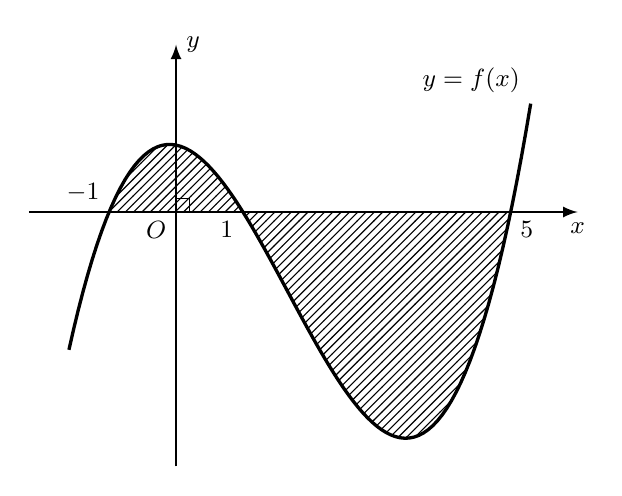
\begin{tikzpicture}[>=latex, scale=0.85]
    % Thư viện cần dùng: \usetikzlibrary{patterns}

    % Hàm số bậc ba dạng: y = 0.2*(x + 1)*(x - 1)*(x - 5)
    % 1. Tô gạch chéo miền giới hạn trên trục hoành (từ x = -1 đến x = 1)
    \fill[pattern=north east lines] 
        plot[domain=-1:1, samples=100] (\x, {0.2*(\x + 1)*(\x - 1)*(\x - 5)}) -- 
        (1,0) -- (-1,0) -- cycle;

    % 2. Tô gạch chéo miền giới hạn dưới trục hoành (từ x = 1 đến x = 5)
    \fill[pattern=north east lines] 
        plot[domain=1:5, samples=100] (\x, {0.2*(\x + 1)*(\x - 1)*(\x - 5)}) -- 
        (5,0) -- (1,0) -- cycle;

    % 3. Trục tọa độ
    \draw[->, thick] (-2.2,0) -- (6.0,0) node[below] {\small $x$};
    \draw[->, thick] (0,-3.8) -- (0,2.5) node[right] {\small $y$};
    \node[below left] at (0,0) {\small $O$};

    % Ký hiệu vuông góc tại gốc tọa độ O
    \draw (0,0.2) -- (0.2,0.2) -- (0.2,0);

    % 4. Đồ thị hàm số y = f(x)
    \draw[very thick, samples=100, domain=-1.6:5.3] 
        plot (\x, {0.2*(\x + 1)*(\x - 1)*(\x - 5)}) 
        node[above left] {\small $y = f(x)$};

    % 5. Đánh dấu các mốc giá trị trên trục Ox
    \node[above left] at (-1,0) {\small $-1$};
    \node[below left] at (1,0) {\small $1$};
    \node[below right] at (5,0) {\small $5$};
\end{tikzpicture}
\end{center}

Mệnh đề nào sau đây đúng?}{%
    \begin{tasks}(2)
        \task \( \displaystyle S = -\int_{-1}^{1} f(x)dx - \int_{1}^{5} f(x)dx \)
        \task \( \displaystyle S = \int_{-1}^{1} f(x)dx + \int_{1}^{5} f(x)dx \)
        \task \( \displaystyle S = \int_{-1}^{1} f(x)dx - \int_{1}^{5} f(x)dx \)
        \task \( \displaystyle S = -\int_{-1}^{1} f(x)dx + \int_{1}^{5} f(x)dx \)
    \end{tasks}
}

% --- CÂU 9 ---
\questionLinesManual{10}{9}{Cho hàm số \( f(x) \) liên tục trên \( \mathbb{R} \). Gọi S là diện tích hình phẳng giới hạn bởi các đường \( y = f(x), y = 0, x = -1, x = 2 \) (như hình vẽ bên). Mệnh đề nào dưới đây đúng?

\begin{center}
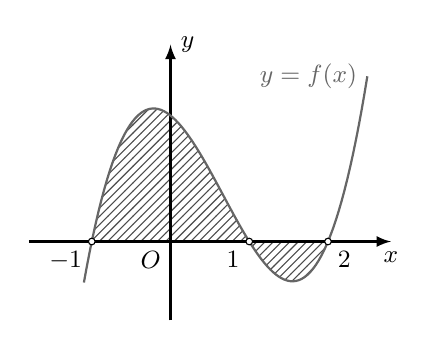
\begin{tikzpicture}[>=latex, scale=1]
    % Thư viện cần dùng: \usetikzlibrary{patterns}

    % Hàm số bậc ba dạng: y = 0.8*(x + 1)*(1 - x)*(x - 2)
    % 1. Tô gạch chéo miền giới hạn trên trục hoành (từ x = -1 đến x = 1)
    \fill[pattern=north east lines, pattern color=black!70] 
        plot[domain=-1:1, samples=100] (\x, {0.8*(\x + 1)*(\x-1)*(\x - 2)}) -- 
        (1,0) -- (-1,0) -- cycle;

    % 2. Tô gạch chéo miền giới hạn dưới trục hoành (từ x = 1 đến x = 2)
    \fill[pattern=north east lines, pattern color=black!70] 
        plot[domain=1:2, samples=100] (\x, {0.8*(\x + 1)*(\x-1)*(\x - 2)}) -- 
        (2,0) -- (1,0) -- cycle;

    % 3. Trục tọa độ
    \draw[->, thick] (-1.8,0) -- (2.8,0) node[below] {\small $x$};
    \draw[->, thick] (0,-1) -- (0,2.5) node[right] {\small $y$};
    \node[below left] at (0,0) {\small $O$};

    % 4. Đồ thị hàm số y = f(x)
    \draw[thick, gray!80!black, samples=100, domain=-1.1:2.5] 
        plot (\x, {0.8*(\x + 1)*(\x-1)*(\x - 2)}) 
        node[left] {\small $y = f(x)$};

    % 5. Đánh dấu các mốc điểm tròn và giá trị trên trục Ox
    \filldraw[fill=white, draw=black] (-1,0) circle (1.2pt) node[below left] {\small $-1$};
    \filldraw[fill=white, draw=black] (1,0) circle (1.2pt) node[below left] {\small $1$};
    \filldraw[fill=white, draw=black] (2,0) circle (1.2pt) node[below right] {\small $2$};
\end{tikzpicture}
\end{center}

Mệnh đề nào dưới đây đúng?}{%
    \begin{tasks}(2)
        \task \( \displaystyle S = \int_{-1}^{1} f(x) dx + \int_{1}^{2} f(x) dx \)
        \task \( \displaystyle S = -\int_{-1}^{1} f(x) dx - \int_{1}^{2} f(x) dx \)
        \task \( \displaystyle S = -\int_{-1}^{1} f(x) dx + \int_{1}^{2} f(x) dx \)
        \task \( \displaystyle S = \int_{-1}^{1} f(x) dx - \int_{1}^{2} f(x) dx \)
    \end{tasks}
}

% --- CÂU 10 ---
\questionLinesManual{10}{10}{Gọi \( S \) là diện tích hình phẳng \( (H) \) giới hạn bởi các đường \( y = f(x) \), trục hoành và hai đường thẳng \( x = -1, \, x = 2 \). Đặt  
\(a = \displaystyle\int_{-1}^{0} f(x) dx, \, b = \int_{0}^{2} f(x) dx,\)
mệnh đề nào sau đây đúng?

\begin{center}
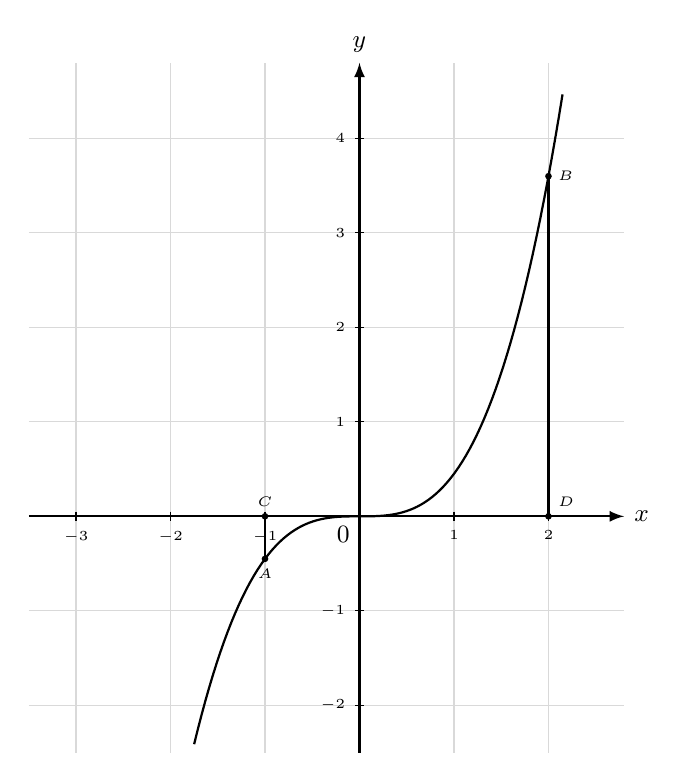
\begin{tikzpicture}[>=latex, scale=1.2]
    % 1. Lưới ô vuông nhạt
    \draw[gray!30, thin] (-3.5,-2.5) grid (2.8,4.8);

    % 2. Trục tọa độ
    \draw[->, thick] (-3.5,0) -- (2.8,0) node[right] {\small $x$};
    \draw[->, thick] (0,-2.5) -- (0,4.8) node[above] {\small $y$};
    \node[below left] at (0,0) {\small $0$};

    % 3. Đánh dấu các mốc trên trục Ox và Oy
    \foreach \x in {-3,-2,-1,1,2} {
        \draw (\x,0.05) -- (\x,-0.05) node[below] {\tiny $\x$};
    }
    \foreach \y in {-2,-1,1,2,3,4} {
        \draw (0.05,\y) -- (-0.05,\y) node[left] {\tiny $\y$};
    }

    % 4. Đồ thị hàm số y = (1/3)*e^x - 1/3 (hoặc y = 1/3*(e^x - 1))
    \draw[thick, samples=100, domain=-1.75:2.15] 
        plot (\x, {0.45*\x*\x*\x});

    % 5. Các đoạn thẳng đứng nối A-C và B-D
    \draw[thick] (-1,0) -- (-1,- 0.45);
    \draw[thick] (2,0) -- (2, 3.6);

    % 6. Các điểm A, B, C, D
    \fill (-1, -0.45) circle (1pt) node[below] {\tiny $A$};
    \fill (2, 3.6) circle (1pt) node[right] {\tiny $B$};
    \fill (-1,0) circle (1pt) node[above] {\tiny $C$};
    \fill (2,0) circle (1pt) node[above right] {\tiny $D$};
\end{tikzpicture}
\end{center}
}{%
    \begin{tasks}(4)
        \task \( S = b - a \)
        \task \( S = b + a \)
        \task \( S = -b + a \)
        \task \( S = -b - a \)
    \end{tasks}
}

% --- CÂU 11 ---
\questionLinesManual{10}{11}{Diện tích phần hình phẳng gạch chéo trong hình vẽ bên được tính theo công thức nào dưới đây?

\begin{center}
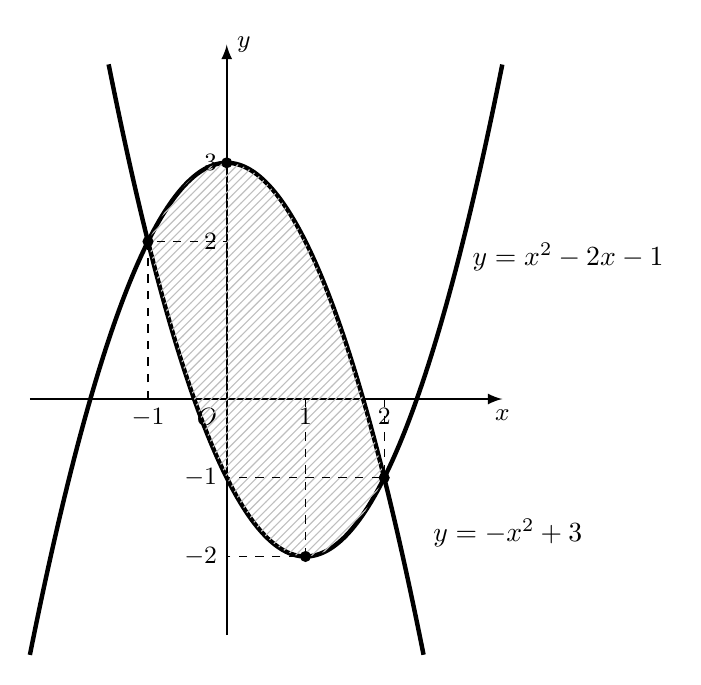
\begin{tikzpicture}[>=latex, scale=1.0]
    % 1. Vẽ hệ trục tọa độ
    \draw[->, black, thick] (-2.5, 0) -- (3.5, 0) node[below] {\small $x$};
    \draw[->, black, thick] (0, -3) -- (0, 4.5) node[right] {\small $y$};
    \node[below left] at (0,0) {\small $O$};
    
    % 2. Vẽ đồ thị hàm số y = x^2 - 2x - 1
    \draw[ultra thick, samples=150, domain=-1.5:3.5] 
        plot (\x, {\x*\x - 2*\x - 1});
    \node[above right] at (3,1.5) {$y = x^2 - 2x - 1$};
    
    % 3. Vẽ đồ thị hàm số y = -x^2 + 3
    \draw[ultra thick, samples=150, domain=-2.5:2.5] 
        plot (\x, {-\x*\x + 3});
    \node[above right] at (2.5,-2) {$y = -x^2 + 3$};
    
    % 4. Tô phần gạch chéo (từ -1 đến 2)
    \fill[pattern=north east lines, pattern color=gray!50, domain=-1:2, variable=\x]
        plot (\x, {-\x*\x + 3}) -- plot (\x, {\x*\x - 2*\x - 1}) -- cycle;
    
    % 5. Đánh dấu các điểm đặc biệt
    \draw[dashed, black] (-1,0) -- (-1,2) -- (0,2);
    \node[below] at (-1,0) {\small $-1$};
    \node[left] at (0,2) {\small $2$};
    \fill (-1,2) circle (2pt);
    
    \draw[dashed, black] (2,0) -- (2,-1) -- (0,-1);
    \node[below] at (2,0) {\small $2$};
    \node[left] at (0,-1) {\small $-1$};
    \fill (2,-1) circle (2pt);
    
    % Đỉnh của parabol y = -x^2 + 3
    \draw[dashed, black] (0,3) -- (0,0);
    \node[left] at (0,3) {\small $3$};
    \fill (0,3) circle (2pt);
    
    % Đỉnh của parabol y = x^2 - 2x - 1
    \draw[dashed, black] (1,0) -- (1,-2) -- (0,-2);
    \node[below] at (1,0) {\small $1$};
    \node[left] at (0,-2) {\small $-2$};
    \fill (1,-2) circle (2pt);
    
\end{tikzpicture}
\end{center}
}{%
    \begin{tasks}(4)
        \task \( \displaystyle\int_{-1}^{2} (-2x + 2) dx \)
        \task \( \displaystyle\int_{-1}^{2} (2x - 2) dx \)
        \task \( \displaystyle\int_{-1}^{2} (-2x^2 + 2x + 4) dx \)
        \task \( \displaystyle\int_{-1}^{2} (2x^2 - 2x - 4) dx \)
    \end{tasks}
}

% --- CÂU 12 ---
\questionLinesManual{10}{12}{Gọi \( S \) là diện tích hình phẳng giới hạn bởi đồ thị hàm số \( y = f(x) \), trục hoành, đường thẳng \( x = a, x = b \) (như hình vẽ bên). Hỏi cách tính \( S \) nào dưới đây đúng?

\begin{center}
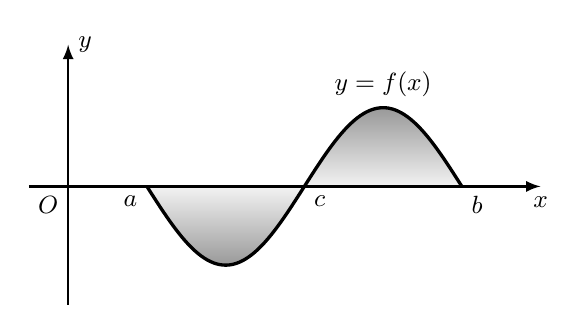
\begin{tikzpicture}[>=latex, scale=1.0]
    % 1. Tô màu xám gradient cho miền âm từ a đến c
    \fill[bottom color=gray!80, top color=gray!10] 
        plot[domain=1:3, samples=100] (\x, {-sin((\x-1)*180/2)}) -- 
        (3,0) -- (1,0) -- cycle;

    % 2. Tô màu xám gradient cho miền dương từ c đến b
    \fill[top color=gray!80, bottom color=gray!10] 
        plot[domain=3:5, samples=100] (\x, {sin((\x-3)*180/2)}) -- 
        (5,0) -- (3,0) -- cycle;

    % 3. Trục tọa độ
    \draw[->, thick] (-0.5,0) -- (6.0,0) node[below] {\small $x$};
    \draw[->, thick] (0,-1.5) -- (0,1.8) node[right] {\small $y$};
    \node[below left] at (0,0) {\small $O$};

    % 4. Đồ thị hàm số y = f(x)
    \draw[very thick, samples=100, domain=1:5] 
        plot (\x, {-sin((\x-1)*180/2)}) 
        node[above]  at (4,1){\small $y = f(x)$};

    % 5. Đánh dấu các mốc giá trị a, c, b trên trục Ox
    \node[below left] at (1,0) {\small $a$};
    \node[below right] at (3,0) {\small $c$};
    \node[below right] at (5,0) {\small $b$};
\end{tikzpicture}
\end{center}
}{%
    \begin{tasks}(2)
        \task \( \displaystyle S = \int_a^b f(x) dx \)
        \task \( \displaystyle S = \left| \int_a^c f(x) dx + \int_c^b f(x) dx \right| \)
        \task \( \displaystyle S = -\int_a^c f(x) dx + \int_c^b f(x) dx \)
        \task \( \displaystyle S = \int_a^c f(x) dx + \int_c^b f(x) dy \)
    \end{tasks}
}

% --- CÂU 13 ---
\questionLinesManual{10}{13}{Cho hàm số \( y = f(x) \) liên tục trên đoạn \([a; b]\). Gọi \( D \) là diện tích hình phẳng giới hạn bởi đồ thị \( (C) : y = f(x) \), trục hoành, hai đường thẳng \( x = a \), \( x = b \) (như hình vẽ dưới đây). Giả sử \( S_D \) là diện tích hình phẳng \( D \). Đúng trong các phương án A, B, C, D cho dưới đây?

\begin{center}
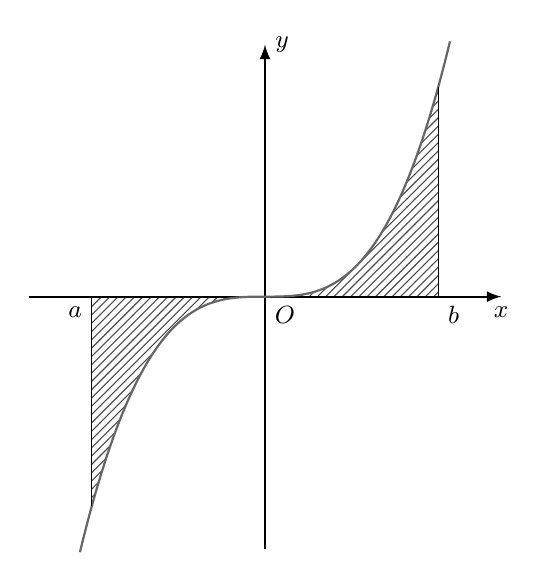
\begin{tikzpicture}[>=latex, scale=1.0]
    % Thư viện cần dùng: \usetikzlibrary{patterns}

    % 1. Tô gạch chéo miền âm từ x = a (-2.2) đến x = 0
    \fill[pattern=north east lines, pattern color=black!70] 
        plot[domain=-2.2:0, samples=100] (\x, {0.25*\x*\x*\x}) -- 
        (0,0) -- (-2.2,0) -- cycle;

    % 2. Tô gạch chéo miền dương từ x = 0 đến x = b (2.2)
    \fill[pattern=north east lines, pattern color=black!70] 
        plot[domain=0:2.2, samples=100] (\x, {0.25*\x*\x*\x}) -- 
        (2.2,0) -- (0,0) -- cycle;

    % 3. Trục tọa độ
    \draw[->, thick] (-3.0,0) -- (3.0,0) node[below] {\small $x$};
    \draw[->, thick] (0,-3.2) -- (0,3.2) node[right] {\small $y$};
    \node[below right] at (0,0) {\small $O$};

    % 4. Đồ thị hàm số (dạng y = k*x^3)
    \draw[thick, gray!80!black, samples=100, domain=-2.35:2.35] 
        plot (\x, {0.25*\x*\x*\x});

    % 5. Các đường dóng đứng tại x = a và x = b
    \draw (-2.2,0) -- (-2.2, {0.25*(-2.2)^3});
    \draw (2.2,0) -- (2.2, {0.25*(2.2)^3});

    % Nhãn hoành độ a, b
    \node[below left] at (-2.2,0) {\small $a$};
    \node[below right] at (2.2,0) {\small $b$};
\end{tikzpicture}
\end{center}
}{%
    \begin{tasks}(2)
        \task \( \displaystyle S_D = \int_a^b f(x) dx + \int_0^b f(x) dx \)
        \task \( \displaystyle S_D = -\int_a^b f(x) dx + \int_0^b f(x) dx \)
        \task \( \displaystyle S_D = \int_a^b f(x) dx - \int_0^b f(x) dx \)
        \task \( \displaystyle S_D = -\int_a^b f(x) dx - \int_0^b f(x) dx \)
    \end{tasks}
}

% --- CÂU 14 ---
\questionLinesManual{10}{14}{Diện tích hình phẳng giới hạn bởi đồ thị hàm số \( y = (x - 2)^2 - 1 \), trục hoành và hai đường thẳng \( x = 1, x = 2 \) bằng}{%
    \begin{tasks}(4)
        \task \( \dfrac{2}{3} \)
        \task \( \dfrac{3}{2} \)
        \task \( \dfrac{1}{3} \)
        \task \( \dfrac{7}{3} \)
    \end{tasks}
}

% --- CÂU 15 ---
\questionLinesManual{10}{15}{Cho hai hàm số \( f(x) \) và \( g(x) \) liên tục trên \([a; b]\). Diện tích hình phẳng giới hạn bởi đồ thị của các hàm số \( y = f(x) \), \( y = g(x) \) và các đường thẳng \( x = a \), \( x = b \) bằng}{%
    \begin{tasks}(4)
        \task \( \displaystyle\int_a^b |f(x) - g(x)| dx \)
        \task \( \displaystyle\int_a^b [f(x) + g(x)] dx \)
        \task \( \displaystyle\int_a^b [f(x) - g(x)] dx \)
        \task \( \displaystyle\int_a^b |f(x) + g(x)| dx \)
    \end{tasks}
}

% --- CÂU 16 ---
\questionLinesManual{10}{16}{Tính diện tích hình phẳng giới hạn bởi đồ thị hàm số \( y = 4x - x^2 \) và trục \( Ox \).}{%
    \begin{tasks}(4)
        \task 11
        \task \( \dfrac{34}{3} \)
        \task \( \dfrac{31}{3} \)
        \task \( \dfrac{32}{3} \)
    \end{tasks}
}

% --- CÂU 17 ---
\questionLinesManual{10}{17}{Diện tích của hình phẳng được giới hạn bởi đồ thị hàm số \( y = f(x) \), trục hoành và hai đường thẳng \( x = a \), \( x = b \) (\( a < b \)) (phần tô đậm trong hình vẽ) tính theo công thức nào dưới đây?

\begin{center}
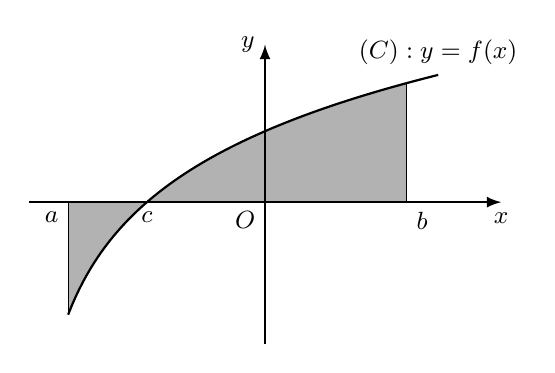
\begin{tikzpicture}[>=latex, scale=1.0]

    % 1. Tô màu xám miền dưới trục hoành (từ x = a đến x = c)
    \fill[gray!60]
        plot[
            domain=-2.5:-1.5,
            samples=100
        ] (\x,{1.3*ln((\x+3)/1.5)}) --
        (-1.5,0) --
        (-2.5,0) --
        cycle;

    % 2. Tô màu xám miền trên trục hoành (từ x = c đến x = b)
    \fill[gray!60]
        plot[
            domain=-1.5:1.8,
            samples=100
        ] (\x,{1.3*ln((\x+3)/1.5)}) --
        (1.8,0) --
        (-1.5,0) --
        cycle;

    % 3. Trục tọa độ
    \draw[->, thick]
        (-3.0,0) -- (3.0,0)
        node[below] {\small $x$};

    \draw[->, thick]
        (0,-1.8) -- (0,2.0)
        node[left] {\small $y$};

    % Gốc tọa độ
    \node[below left] at (0,0) {\small $O$};

    % 4. Đồ thị hàm số (C): y = f(x)
    \draw[
        thick,
        samples=100,
        domain=-2.5:2.2
    ]
        plot (\x,{1.3*ln((\x+3)/1.5)})
        node[above ]
        {\small $(C): y=f(x)$};

    % 5. Đánh dấu các ranh giới đứng tại x = a và x = b
    \draw
        (-2.5,0) --
        (-2.5,{1.3*ln((-2.5+3)/1.5)});

    \draw
        (1.8,0) --
        (1.8,{1.3*ln((1.8+3)/1.5)});

    % 6. Nhãn các điểm a, c, b
    \node[below left] at (-2.5,0) {\small $a$};

    \node[below] at (-1.5,0) {\small $c$};

    \node[below right] at (1.8,0) {\small $b$};

\end{tikzpicture}
\end{center}
}{%
    \begin{tasks}(2)
        \task \( \displaystyle S = \int_a^b f(x) dx + \int_c^b f(x) dx \)
        \task \( \displaystyle S = \int_a^b f(x) dx \)
        \task \( \displaystyle S = -\int_a^c f(x) dx + \int_c^b f(x) dx \)
        \task \( \displaystyle S = \left| \int_a^b f(x) dx \right| \)
    \end{tasks}
}

% --- CÂU 18 ---
\questionLinesManual{10}{18}{Gọi diện tích hình phẳng giới hạn bởi đồ thị hàm số  
\[(C): y = \frac{-3x - 1}{x - 1}\]
và hai trục tọa độ là \( S \). Tính \( S \)?}{%
    \begin{tasks}(4)
        \task \( S = 1 - \ln \dfrac{4}{3} \)
        \task \( S = 4 \ln \dfrac{4}{3} \)
        \task \( S = 4 \ln \dfrac{4}{3} - 1 \)
        \task \( S = \ln \dfrac{4}{3} - 1 \)
    \end{tasks}
}

% --- CÂU 19 ---
\questionLinesManual{10}{19}{Diện tích hình phẳng giới hạn bởi \( y = x^2; y = 0; x = 1; x = 2 \) bằng}{%
    \begin{tasks}(4)
        \task \( \dfrac{4}{3} \)
        \task \( \dfrac{7}{3} \)
        \task \( \dfrac{8}{3} \)
        \task 1
    \end{tasks}
}

% --- CÂU 20 ---
\questionLinesManual{10}{20}{Gọi \( S \) là diện tích hình phẳng giới hạn bởi đồ thị của hàm số  
\[(H): y = \frac{x - 1}{x + 1}\]
và các trục tọa độ. Khi đó giá trị của \( S \) bằng}{%
    \begin{tasks}(4)
        \task \( 2 \ln 2 - 1 \)
        \task \( \ln 2 + 1 \)
        \task \( \ln 2 - 1 \)
        \task \( 2 \ln 2 + 1 \)
    \end{tasks}
}

% --- CÂU 21 ---
\questionLinesManual{10}{21}{Diện tích hình phẳng giới hạn bởi hai đồ thị hàm số \( y = x^3 \), \( y = x^2 - 4x + 4 \) và trục \( Ox \) (tham khảo hình vẽ) được tính theo công thức nào dưới đây?

\begin{center}
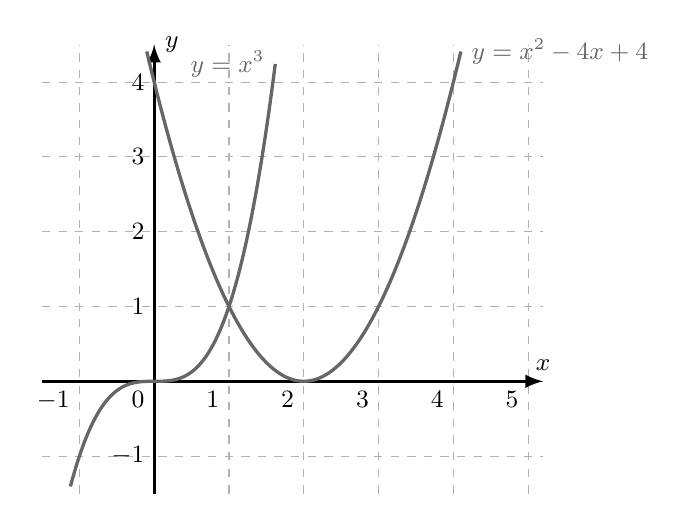
\begin{tikzpicture}[>=latex, scale=0.95]
    % 1. Lưới ô vuông nét đứt
    \draw[dashed, gray!60, thin] (-1.5,-1.5) grid (5.2,4.5);

    % 2. Trục tọa độ
    \draw[->, very thick] (-1.5,0) -- (5.2,0) node[above] {\small $x$};
    \draw[->, very thick] (0,-1.5) -- (0,4.5) node[right] {\small $y$};
    \node[below left] at (0,0) {\small $0$};

    % 3. Đánh dấu các mốc giá trị trên hai trục
    \foreach \x in {-1,1,2,3,4,5} {
        \node[below left] at (\x,0) {\small $\x$};
    }
    \foreach \y in {-1,1,2,3,4} {
        \node[left] at (0,\y) {\small $\y$};
    }

    % 4. Đồ thị các hàm số
    % Hàm bậc ba y = x^3
    \draw[very thick, gray!80!black, samples=100, domain=-1.12:1.62] 
        plot (\x, {(\x)^3}) 
        node[left] {\small $y = x^3$};

    % Parabol y = x^2 - 4x + 4
    \draw[very thick, gray!80!black, samples=100, domain=-0.1:4.1] 
        plot (\x, {(\x)^2 - 4*\x + 4}) 
        node[right] {\small $y = x^2 - 4x + 4$};
\end{tikzpicture}
\end{center}
}{%
    \begin{tasks}(2)
        \task \( \displaystyle\int_{0}^{2} x^3 - (x^2 - 4x + 4) dx \)
        \task \( \displaystyle\int_{0}^{2} x^3 dx - \int_{0}^{2} (x^2 - 4x + 4) dx \)
        \task \( \displaystyle\int_{0}^{2} x^3 dx - \int_{0}^{2} (x^2 - 4x + 4) dx \)
        \task \( \displaystyle\int_{0}^{2} x^3 dx + \int_{0}^{2} (x^2 - 4x + 4) dx \)
    \end{tasks}
}

% --- CÂU 22 ---
\questionLinesManual{10}{22}{Viết công thức tính thể tích \( V \) của khối tròn xoay được tạo ra khi quay hình thang cong, giới hạn bởi đồ thị hàm số \( y = f(x) \), trục \( Ox \) và hai đường thẳng \( x = a, x = b (a < b) \), xung quanh trục \( Ox \).}{%
    \begin{tasks}(4)
        \task \( \displaystyle V = \int_a^b |f(x)| dx \)
        \task \( \displaystyle V = \pi \int_a^b f^2(x) dx \)
        \task \( \displaystyle V = \int_a^b f^2(x) dx \)
        \task \( \displaystyle V = \pi \int_a^b f(x) dx \)
    \end{tasks}
}

% --- CÂU 23 ---
\questionLinesManual{10}{23}{Cho hàm số \( y = f(x) \) liên tục trên đoạn \([a; b]\). Gọi \( D \) là hình phẳng giới hạn bởi đồ thị hàm số \( y = f(x) \), trục hoành và hai đường thẳng \( x = a, x = b (a < b) \). Thể tích của khối tròn xoay tạo thành khi quay \( D \) quanh trục hoành được tính theo công thức:}{%
    \begin{tasks}(4)
        \task \( \displaystyle V = \pi \int_a^b f(x) dx \)
        \task \( \displaystyle V = \pi \int_a^b f^2(x) dx \)
        \task \( \displaystyle V = 2\pi \int_a^b f^2(x) dx \)
        \task \( \displaystyle V = \pi \int_a^b f^2(x) dx \)
    \end{tasks}
}

% --- CÂU 24 ---
\questionLinesManual{10}{24}{Gọi \( D \) là hình phẳng giới hạn bởi các đường \( y = e^{3x}, y = 0, x = 0 \) và \( x = 1 \). Thể tích của khối tròn xoay tạo thành khi quay \( D \) quanh trục \( Ox \) bằng:}{%
    \begin{tasks}(4)
        \task \( \displaystyle \pi \int_0^1 e^{3x} dx \)
        \task \( \displaystyle \int_0^1 e^{6x} dx \)
        \task \( \displaystyle \pi \int_0^1 e^{6x} dx \)
        \task \( \displaystyle \int_0^1 e^{3x} dx \)
    \end{tasks}
}

% --- CÂU 25 ---
\questionLinesManual{10}{25}{Gọi \( D \) là hình phẳng giới hạn bởi các đường \( y = e^{4x}, y = 0, x = 0 \) và \( x = 1 \). Thể tích của khối tròn xoay tạo thành khi quay \( D \) quanh trục \( Ox \) bằng:}{%
    \begin{tasks}(4)
        \task \( \displaystyle \int_0^1 e^{4x} dx \)
        \task \( \displaystyle \pi \int_0^1 e^{8x} dx \)
        \task \( \displaystyle \int_0^1 e^{8x} dx \)
        \task \( \displaystyle \pi \int_0^1 e^{4x} dx \)
    \end{tasks}
}

% --- CÂU 26 ---
\questionLinesManual{10}{26}{Cho hình phẳng \( (H) \) giới hạn bởi các đường \( y = x^2 + 3 \), \( y = 0 \), \( x = 0 \), \( x = 2 \).  
Gọi \( V \) là thể tích của khối tròn xoay được tạo thành khi quay \( (H) \) xung quanh trục \( Ox \). Mệnh đề nào dưới đây đúng?}{%
    \begin{tasks}(4)
        \task \( \displaystyle V = \int_0^2 (x^2 + 3) dx \)
        \task \( \displaystyle V = \pi \int_0^2 (x^2 + 3) dx \)
        \task \( \displaystyle V = \int_0^2 (x^2 + 3)^2 dx \)
        \task \( \displaystyle V = \pi \int_0^2 (x^2 + 3)^2 dx \)
    \end{tasks}
}

% --- CÂU 27 ---
\questionLinesManual{10}{27}{Cho hình phẳng \( D \) giới hạn bởi đường cong \( y = e^x \), trục hoành và các đường thẳng \( x = 0 \), \( x = 1 \). Khối tròn xoay tạo thành khi quay \( D \) quanh trục hoành có thể tích \( V \) bằng bao nhiêu?}{%
    \begin{tasks}(4)
        \task \( \displaystyle V = \dfrac{\pi (e^2 + 1)}{2} \)
        \task \( \displaystyle V = \dfrac{e^2 - 1}{2} \)
        \task \( \displaystyle V = \dfrac{\pi e^2}{3} \)
        \task \( \displaystyle V = \dfrac{\pi (e^2 - 1)}{2} \)
    \end{tasks}
}

% --- CÂU 28 ---
\questionLinesManual{10}{28}{Cho hình phẳng \( D \) giới hạn với đường cong \( y = \sqrt{x^2 + 1} \), trục hoành và các đường thẳng \( x = 0 \), \( x = 1 \). Khối tròn xoay tạo thành khi quay \( D \) quanh trục hoành có thể tích \( V \) bằng bao nhiêu?}{%
    \begin{tasks}(4)
        \task \( \displaystyle V = 2 \)
        \task \( \displaystyle V = \dfrac{4\pi}{3} \)
        \task \( \displaystyle V = 2\pi \)
        \task \( \displaystyle V = \dfrac{4}{3} \)
    \end{tasks}
}

% --- CÂU 29 ---
\questionLinesManual{10}{29}{Tính thể tích V của phần vật thể giới hạn bởi hai mặt phẳng \( x = 1 \) và \( x = 3 \), biết rằng khi cắt vật thể bởi mặt phẳng vuông góc với trục \( Ox \) tại điểm có hoành độ \( x \) (\( 1 \leq x \leq 3 \)) thì được thiết diện là một hình chữ nhật có độ dài hai cạnh là \( 3x \) và \( \sqrt{3x^2 - 2} \).}{%
    \begin{tasks}(4)
        \task \( V = \dfrac{124}{3} \)
        \task \( V = (32 + 2\sqrt{15})\pi \)
        \task \( V = 32 + 2\sqrt{15} \)
        \task \( V = \dfrac{124\pi}{3} \)
    \end{tasks}
}

% --- CÂU 30 ---
\questionLinesManual{10}{30}{Tìm công thức tính thể tích của khối tròn xoay khi cho hình phẳng giới hạn bởi parabol  
\((P): y = x^2\) và đường thẳng \(d: y = 2x\) quay xung quanh trục \( Ox \).}{%
    \begin{tasks}(4)
        \task \( \displaystyle \pi \int_{0}^{2} (x^2 - 2x)^2 dx \)
        \task \( \displaystyle \pi \int_{0}^{2} 4x^2 dx - \pi \int_{0}^{2} x^4 dx \)
        \task \( \displaystyle \pi \int_{0}^{2} 4x^2 dx + \pi \int_{0}^{2} x^4 dx \)
        \task \( \displaystyle \pi \int_{0}^{2} (2x - x^2) dx \)
    \end{tasks}
}

% --- CÂU 31 ---
\questionLinesManual{10}{31}{Khi cắt vật thể bởi mặt phẳng vuông góc với trục \( Ox \) tại điểm có hoành độ là \( x \), \( (0 \leq x \leq 3) \) ta được mặt cắt là một hình vuông có cạnh là \( \sqrt{9 - x^2} \) (được mô hình hóa bởi hình vẽ bên dưới). Thể tích của vật thể đó bằng

\begin{center}
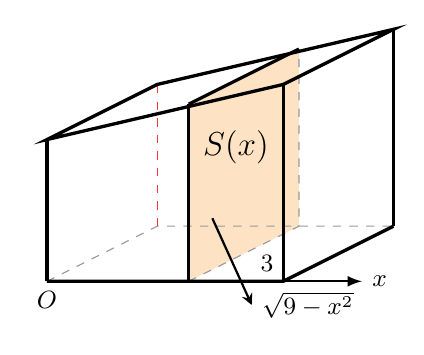
\begin{tikzpicture}[scale=1.0, >=latex]
    % Định nghĩa màu tô thiết diện S(x)
    \definecolor{secfill}{RGB}{253, 226, 195}

    % 1. Tô màu thiết diện S(x)
    \fill[secfill] (1.8, 0) -- (1.8, 2.25) -- (3.2, 2.95) -- (3.2, 0.7) -- cycle;

    % 2. Đường nét đứt phía sau
    \draw[dashed, gray!80] (0, 0) -- (1.4, 0.7) -- (4.4, 0.7);
    \draw[dashed, red!80] (1.4, 0.7) -- (1.4, 2.5); % Cạnh đứng đứt màu đỏ
    \draw[dashed, gray!80] (1.8, 0) -- (3.2, 0.7) -- (3.2, 2.95); % Cạnh của thiết diện S(x)
    \draw[dashed, gray!80] (4.4, 0.7) -- (4.4, 3.2);

    % 3. Đường nét liền vật thể
    % Mặt đáy
    \draw[very thick] (0,0) -- (3,0) -- (4.4, 0.7);
    \draw[very thick] (0,0) -- (0, 1.8);
    % Mặt bên trước và các cạnh đứng
    \draw[very thick] (3,0) -- (3, 2.5);
    \draw[very thick] (4.4,0.7) -- (4.4, 3.2);
    % Mặt trên
    \draw[very thick] (0, 1.8) -- (1.4, 2.5) -- (4.4, 3.2) -- (3, 2.5) -- cycle;
    
    % Cạnh trước thiết diện S(x)
    \draw[very thick] (1.8,0) -- (1.8, 2.25);
    \draw[very thick] (1.8, 2.25) -- (3.2, 2.95);

    % 4. Trục Ox và các ký hiệu
    \draw[->, thick] (3,0) -- (4.0,0) node[right] {\small $x$};
    
  

    % Nhãn text
    \node[below] at (0,0) {\small $O$};
    \node[above left] at (3,0) {\small $3$};
    \node at (2.4, 1.7) {\large $S(x)$};

    % Mũi tên chỉ kích thước căn(9 - x^2)
    \draw[->, >=stealth, thick] (2.1, 0.8) -- (2.6, -0.3) node[right] {\small $\sqrt{9-x^2}$};
\end{tikzpicture}
\end{center}
}{%
    \begin{tasks}(4)
        \task \( 171\pi \)
        \task \( 171 \)
        \task \( 18\pi \)
        \task \( 18 \)
    \end{tasks}
}

% --- CÂU 32 ---
\questionLinesManual{10}{32}{Tính thể tích \( V \) của vật thể giới hạn bởi hai mặt phẳng \( x = 0 \) và \( x = 1 \), biết rằng khi cắt vật thể bởi mặt phẳng tùy ý vuông góc với trục \( Ox \) tại điểm có hoành độ \( x(0 \leq x \leq 1) \) thì được thiết diện là hình vuông có cạnh bằng \( (x + 1) \).}{%
    \begin{tasks}(4)
        \task \( V = \dfrac{3\pi}{2} \)
        \task \( V = \dfrac{7\pi}{3} \)
        \task \( V = \dfrac{7}{3} \)
        \task \( V = \dfrac{3}{2} \)
    \end{tasks}
}

% --- CÂU 33 ---
\questionLinesManual{10}{33}{Cho phần vật thể \( (T) \) giới hạn bởi hai mặt phẳng có phương trình \( x = 0 \) và \( x = 2 \). Cắt phần vật thể \( (T) \) bởi mặt phẳng vuông góc với trục \( Ox \) tại điểm có hoành độ \( x(0 \leq x \leq 2) \), ta được thiết diện là một tam giác đều có độ dài cạnh bằng \( x\sqrt{2 - x} \). Tính thể tích \( V \) của phần vật thể \( (T) \).}{%
    \begin{tasks}(4)
        \task \( V = \dfrac{\sqrt{3}}{2} \)
        \task \( V = \dfrac{\sqrt{3}}{3} \)
        \task \( V = \dfrac{\sqrt{3}\pi}{2} \)
        \task \( V = \dfrac{\sqrt{3}\pi}{3} \)
    \end{tasks}
}

% --- CÂU 34 ---
\questionLinesManual{10}{34}{Gọi \( S \) là diện tích của hình phẳng giới hạn bởi các đường \( y = 2x^2 + 3x - 5 \), \( y = 0 \), \( x = -2 \), \( x = 3 \). Mệnh đề nào dưới đây đúng?}{%
    \begin{tasks}(4)
        \task \( \displaystyle S = \int_{-2}^{3} (2x^2 + 3x - 5) dx \)
        \task \( \displaystyle S = \int_{-\frac{5}{2}}^{\frac{1}{2}} (2x^2 + 3x - 5) dx \)
        \task \( \displaystyle S = \int_{-2}^{3} (2x^2 + 3x - 5) dx \)
        \task \( \displaystyle S = \int_{-\frac{5}{2}}^{-\frac{1}{2}} (2x^2 + 3x - 5) dx \)
    \end{tasks}
}

% --- CÂU 35 ---
\questionLinesManual{10}{35}{Cho hình phẳng \( (H) \) giới hạn bởi các đường \( y = -x^2 + 1 \), \( y = 0 \), \( x = -2 \), \( x = 3 \). Gọi \( V \) là thể tích của khối tròn xoay được tạo thành khi quay \( (H) \) xung quanh trục \( Ox \). Mệnh đề nào dưới đây đúng?}{%
    \begin{tasks}(4)
        \task \( \displaystyle V = \pi \int_{-2}^{3} (-x^2 + 1) dx \)
        \task \( \displaystyle V = \int_{-2}^{3} (-x^2 + 1)^2 dx \)
        \task \( \displaystyle V = \int_{-2}^{3} (-x^2 + 1) dx \)
        \task \( \displaystyle V = \pi \int_{-2}^{3} (-x^2 + 1)^2 dx \)
    \end{tasks}
}

% --- CÂU 36 ---
\questionLinesManual{10}{36}{Trong hệ trục tọa độ \( Oxy \), diện tích \( S \) của hình phẳng giới hạn bởi đồ thị hàm số \( y = f(x) \), \( f(x) \geq 0, \, \forall x \in [0; 2] \), trục \( Ox, Oy \), đường thẳng \( x = 2 \) là \( 3 \). Tính \( \displaystyle\int_{0}^{2} f(x) dx \).}{%
    \begin{tasks}(4)
        \task \( 9\pi \)
        \task \( 3\pi \)
        \task \( 3 \)
        \task \(-3\)
    \end{tasks}
}

% --- CÂU 37 ---
\questionLinesManual{10}{37}{Tính diện tích \( S \) của hình phẳng giới hạn bởi đồ thị hàm số \( y = x^3 - 2 \), trục hoành, trục tung và đường thẳng \( x = 1 \)?}{%
    \begin{tasks}(4)
        \task \( \displaystyle S = \int_{0}^{1} (2 - x^3) dx \)
        \task \( \displaystyle S = \int_{0}^{1} (x^3 - 2)^2 dx \)
        \task \( \displaystyle S = \int_{0}^{1} (x^3 - 2) dx \)
        \task \( \displaystyle S = \pi \int_{0}^{1} (x^3 - 2)^2 dx \)
    \end{tasks}
}

% --- CÂU 38 ---
\questionLinesManual{10}{38}{Cho hình phẳng giới hạn bởi các đường \( y = 1 - \sqrt{x} \), trục hoành và \( x = 9 \) quay xung quanh trục \( Ox \). Tính thể tích khối tròn xoay tạo thành.}{%
    \begin{tasks}(4)
        \task \( V = \dfrac{27\pi}{2} \)
        \task \( V = 13\pi \)
        \task \( V = \dfrac{41\pi}{3} \)
        \task \( V = \dfrac{40\pi}{3} \)
    \end{tasks}
}

% --- CÂU 39 ---
\questionLinesManual{10}{39}{Gọi \( (H) \) là hình phẳng giới hạn bởi hàm số \( y = \sqrt{x+1} \), trục hoành và các đường thẳng \( x = -1, x = 2 \). Thể tích \( V \) của khối tròn xoay tạo thành khi quay \( (H) \) xung quanh trục \( Ox \) được tính bởi công thức nào dưới đây?}{%
    \begin{tasks}(4)
        \task \( \displaystyle V = \pi \int_{-1}^{2} (x+1) dx \)
        \task \( \displaystyle V = \pi \int_{-1}^{2} \sqrt{x+1} dx \)
        \task \( \displaystyle V = \pi^2 \int_{-1}^{2} \sqrt{x+1} dx \)
        \task \( \displaystyle V = \pi^2 \int_{-1}^{2} (x+1) dx \)
    \end{tasks}
}

% --- CÂU 40 ---
\questionLinesManual{10}{40}{Cho \( (H) \) là hình phẳng giới hạn bởi parabol \( y = \sqrt{3}x^2 \), cung tròn có phương trình \( y = \sqrt{4 - x^2} \) (với \( 0 \le x \le 2 \)) và trục hoành (phần tô đậm trong hình vẽ). Diện tích của \( (H) \) bằng

\begin{center}
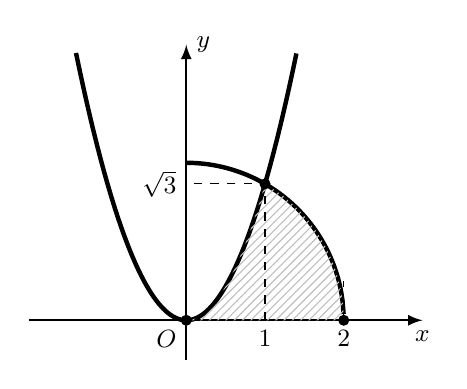
\begin{tikzpicture}[>=latex, scale=1.0]
    % 1. Vẽ hệ trục tọa độ
    \draw[->, black, thick] (-2, 0) -- (3, 0) node[below] {\small $x$};
    \draw[->, black, thick] (0, -0.5) -- (0, 3.5) node[right] {\small $y$};
    \node[below left] at (0,0) {\small $O$};
    
    % 2. Vẽ parabol y = sqrt(3)*x^2
    \draw[ultra thick, samples=150, domain=-1.4:1.4] 
        plot (\x, {1.732*\x*\x});
    
    \draw[ultra thick, samples=150, domain=0:2] 
        plot (\x, {sqrt(4 - \x*\x)});
    
    \fill[pattern=north east lines, pattern color=gray!50] 
        plot[domain=0:1, samples=100] (\x, {1.732*\x*\x}) -- 
        plot[domain=1:0, samples=100] (\x, {0}) -- cycle;
    
    % 5. Tô phần diện tích (phần tô đậm từ x = 1 đến x = 2)
    \fill[pattern=north east lines, pattern color=gray!50] 
        plot[domain=1:2, samples=100] (\x, {sqrt(4 - \x*\x)}) -- 
        plot[domain=2:1, samples=100] (\x, {0}) -- cycle;
    
    % 6. Đánh dấu các điểm đặc biệt
    % Giao điểm của parabol và cung tròn tại x = 1
    \draw[dashed, black] (1,0) -- (1,1.732) -- (0,1.732);
    \node[below] at (1,0) {\small $1$};
    \node[left] at (0,1.732) {\small $\sqrt{3}$};
    \fill (1,1.732) circle (2pt);
    
    % Giao điểm của cung tròn với trục Ox tại x = 2
    \draw[dashed, black] (2,0) -- (2,0.5);
    \node[below] at (2,0) {\small $2$};
    \fill (2,0) circle (2pt);
    
    % Gốc tọa độ O
    \fill (0,0) circle (2pt);
    
\end{tikzpicture}
\end{center}
}{%
    \begin{tasks}(4)
        \task \( \dfrac{4\pi + \sqrt{3}}{12} \)
        \task \( \dfrac{4\pi - \sqrt{3}}{6} \)
        \task \( \dfrac{4\pi + 2\sqrt{3} - 3}{6} \)
        \task \( \dfrac{5\sqrt{3} - 2\pi}{3} \)
    \end{tasks}
}

% --- CÂU 41 ---
\questionLinesManual{10}{41}{Diện tích hình phẳng giới hạn bởi đường cong \( y = x \ln x \), trục hoành và đường thẳng \( x = e \) là}{%
    \begin{tasks}(4)
        \task \( \dfrac{e^2 - 1}{2} \)
        \task \( \dfrac{e^2 + 1}{2} \)
        \task \( \dfrac{e^2 - 1}{4} \)
        \task \( \dfrac{e^2 + 1}{4} \)
    \end{tasks}
}

% --- CÂU 42 ---
\questionLinesManual{10}{42}{Tính diện tích \( S \) của hình phẳng \( (H) \) giới hạn bởi các đường cong \( y = -x^3 + 12x \) và \( y = -x^2 \).}{%
    \begin{tasks}(4)
        \task \( S = \dfrac{937}{12} \)
        \task \( S = \dfrac{343}{12} \)
        \task \( S = \dfrac{793}{4} \)
        \task \( S = \dfrac{397}{4} \)
    \end{tasks}
}

% --- CÂU 43 ---
\questionLinesManual{10}{43}{Cho hình phẳng \( (H) \) giới hạn bởi parabol \( y = \dfrac{x^2}{12} \) và đường cong có phương trình \( y = \sqrt{4 - \dfrac{x^2}{4}} \) (tham khảo hình vẽ bên)

\begin{center}
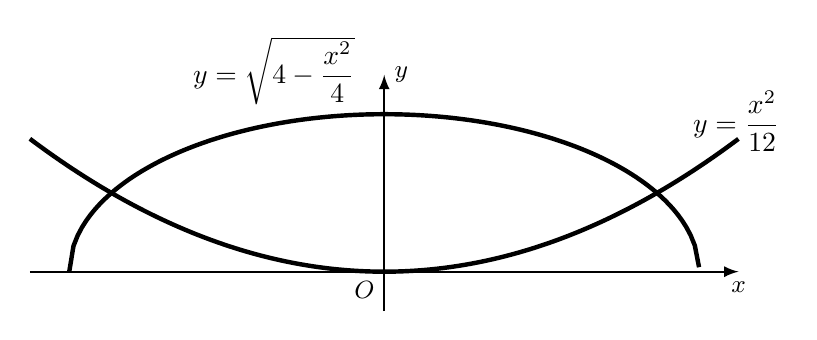
\begin{tikzpicture}[>=latex, scale=1.0]
    % 1. Vẽ hệ trục tọa độ
    \draw[->, black, thick] (-4.5, 0) -- (4.5, 0) node[below] {\small $x$};
    \draw[->, black, thick] (0, -0.5) -- (0, 2.5) node[right] {\small $y$};
    \node[below left] at (0,0) {\small $O$};
    
    % 2. Vẽ parabol y = x^2/12
    \draw[ultra thick, samples=150, domain=-4.5:4.5] 
        plot (\x, {\x*\x/12});
    \node[above right] at (3.8,1.4) {$y = \dfrac{x^2}{12}$};
    
    % 3. Vẽ đường cong y = sqrt(4 - x^2/4)
    \draw[ultra thick, samples=150, domain=-4:4] 
        plot (\x, {sqrt(4 - \x*\x/4)});
    \node[above] at (-1.4,2) {$y = \sqrt{4 - \dfrac{x^2}{4}}$};
    
\end{tikzpicture}
\end{center}

Diện tích hình phẳng \( (H) \) bằng:}{%
    \begin{tasks}(4)
        \task \( 2\left(4\pi + \sqrt{3}\right) \)
        \task \( \dfrac{4\pi + \sqrt{3}}{6} \)
        \task \( \dfrac{4\pi + \sqrt{3}}{3} \)
        \task \( \dfrac{4\sqrt{3} + \pi}{6} \)
    \end{tasks}
}

% --- CÂU 44 ---
\questionLinesManual{10}{44}{Gọi \( V \) là thể tích khối tròn xoay tạo thành do quay xung quanh trục hoành một elip có phương trình  
\[\frac{x^2}{25} + \frac{y^2}{16} = 1.\]
\( V \) có giá trị gần nhất với giá trị nào sau đây?}{%
    \begin{tasks}(4)
        \task 550
        \task 400
        \task 670
        \task 335
    \end{tasks}
}

% --- CÂU 45 ---
\questionLinesManual{10}{45}{Hình vuông \( OABC \) có cạnh bằng 4 được chia thành hai phần bởi đường cong \( (C) \) có phương trình  
\(y = \dfrac{1}{4}x^2.\)
Gọi \( S_1, S_2 \) lần lượt là diện tích của phần không bị gạch và bị gạch như hình vẽ bên dưới. Tỉ số  
\(\dfrac{S_1}{S_2}\)
bằng

\begin{center}
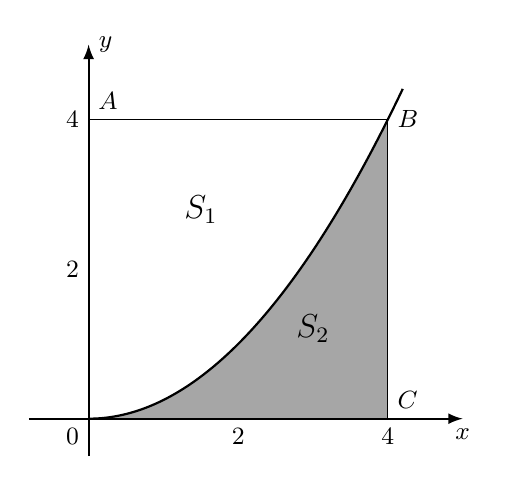
\begin{tikzpicture}[>=latex, scale=0.95]
    % 1. Tô màu xám miền S2
    \fill[gray!70] 
        plot[domain=0:4, samples=100] (\x, {0.25*\x*\x}) -- 
        (4,0) -- (0,0) -- cycle;

    % 2. Trục tọa độ
    \draw[->, thick] (-0.8,0) -- (5,0) node[below] {\small $x$};
    \draw[->, thick] (0,-0.5) -- (0,5) node[right] {\small $y$};
    \node[below left] at (0,0) {\small $0$};

    % 3. Khung hình chữ nhật OABC
    \draw (0,4) -- (4,4) -- (4,0);

    % 4. Đồ thị hàm số y = 1/4 * x^2
    \draw[thick, samples=100, domain=0:4.2] 
        plot (\x, {0.25*\x*\x});

    % 5. Đánh dấu các mốc giá trị trên hai trục
    \node[left] at (0,2) {\small $2$};
    \node[left] at (0,4) {\small $4$};

    \node[below] at (2,0) {\small $2$};
    \node[below] at (4,0) {\small $4$};

    % 6. Nhãn các điểm và miền diện tích
    \node[above right] at (0,4) {\small $A$};
    \node[ right] at (4,4) {\small $B$};
    \node[above right] at (4,0) {\small $C$};

    \node at (1.5, 2.8) {\large $S_1$};
    \node at (3.0, 1.2) {\large $S_2$};
\end{tikzpicture}
\end{center}
}{%
    \begin{tasks}(4)
        \task \( \dfrac{3}{2} \)
        \task 3
        \task \( \dfrac{1}{2} \)
        \task 2
    \end{tasks}
}

% --- CÂU 46 ---
\questionShortAnswer{20}{46}{Gọi \( (H) \) là phần hình phẳng giới hạn bởi đồ thị \( (C) \) của hàm số đa thức bậc ba với đồ thị \( (P) \) của hàm số bậc hai (phần tô đậm) như hình vẽ bên. Tính diện tích của hình phẳng \( (H) \).

\begin{center}
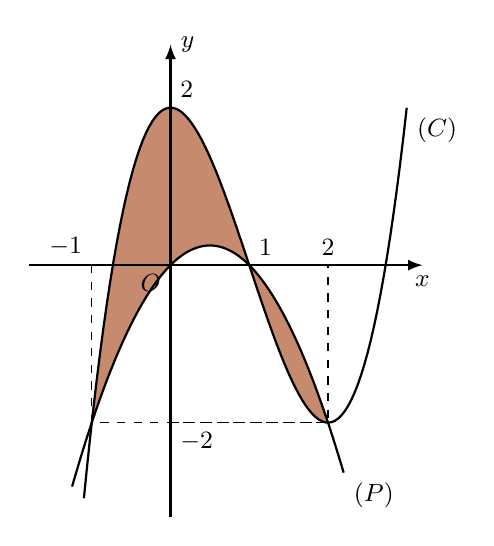
\begin{tikzpicture}[>=latex, scale=1.0]
    % Định nghĩa màu nâu cho miền tô
    \definecolor{brownfill}{RGB}{198, 138, 110}
    \fill[brownfill] 
        plot[domain=-1:2, samples=100] (\x, {\x*\x*\x - 3*\x*\x + 2}) -- 
        plot[domain=2:-1, samples=100] (\x, {-\x*\x + \x}) -- cycle;

    % 2. Trục tọa độ
    \draw[->, thick] (-1.8,0) -- (3.2,0) node[below] {\small $x$};
    \draw[->, thick] (0,-3.2) -- (0,2.8) node[right] {\small $y$};
    \node[below left] at (0,0) {\small $O$};

    % 3. Đồ thị đường cong (C)
    \draw[thick, samples=100, domain=-1.1:3] 
        plot (\x, {\x*\x*\x - 3*\x*\x + 2}) 
        node[below right] {\small $(C)$};

    % 4. Đồ thị parabol (P)
    \draw[thick, samples=100, domain=-1.25:2.2] 
        plot (\x, {-\x*\x + \x}) 
        node[below right] {\small $(P)$};

    % 5. Đường gióng nét đứt và nhãn tọa độ
    \draw[dashed] (-1,0) -- (-1,-2) -- (2,-2) -- (2,0);
    \draw[dashed] (0,-2) -- (2,-2);

    \node[above left] at (-1,0) {\small $-1$};
    \node[above right] at (1,0) {\small $1$};
    \node[above] at (2,0) {\small $2$};
    \node[above right] at (0,2) {\small $2$};
    \node[below right] at (0,-2) {\small $-2$};
\end{tikzpicture}
\end{center}
}

\questionShortAnswer{20}{47}{Cho khối tròn xoay như Hình. Tính thể tích của khối tròn xoay được tạo thành bởi hình phẳng cho ở Hình khi quay quanh trục \( Ox \) (viết kết quả dưới dạng số thập phân và làm tròn đến hàng phần mười).

\begin{center}
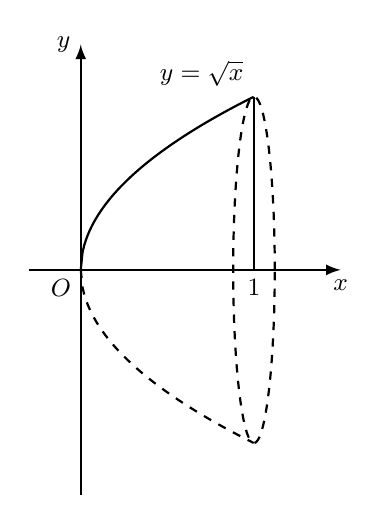
\begin{tikzpicture}[>=latex, scale=2.2]
    % 1. Trục tọa độ
    \draw[->, thick] (-0.3,0) -- (1.5,0) node[below] {\small $x$};
    \draw[->, thick] (0,-1.3) -- (0,1.3) node[left] {\small $y$};
    \node[below left] at (0,0) {\small $O$};

    % 2. Đồ thị phía trên: y = sqrt(x)
    \draw[thick, samples=100, domain=0:1] 
        plot (\x, {sqrt(\x)}) 
        node[above left] {\small $y = \sqrt{x}$};

    % 3. Đồ thị nét đứt đối xứng phía dưới: y = -sqrt(x)
    \draw[dashed, thick, samples=100, domain=0:1] 
        plot (\x, {-sqrt(\x)});

    % 4. Mặt đáy elip biểu diễn khối tròn xoay tại x = 1
    \draw[dashed, thick] (1,0) ellipse (0.12cm and 1cm);

    % 5. Đoạn thẳng đứng nối từ trục Ox lên đỉnh tại x = 1
    \draw[thick] (1,0) -- (1,1);

    % 6. Nhãn giá trị tại x = 1
    \node[below ] at (1,0) {\small $1$};
\end{tikzpicture}
\end{center}
}

\questionShortAnswer{20}{48}{Một khối bê tông cao 2 m được đặt trên mặt đất phẳng. Nếu cắt khối bê tông này bằng mặt phẳng nằm ngang, cách mặt đất \( x(m) \) (\(0 \le x \le 2\)) thì được mặt cắt là hình chữ nhật có chiều dài 5 m, chiều rộng \( (0,5)^x(m) \) (Hình). Tính thể tích của khối bê tông (kết quả làm tròn đến hàng phần trăm của mét khối).
\begin{figure}[htbp]
    \centering
    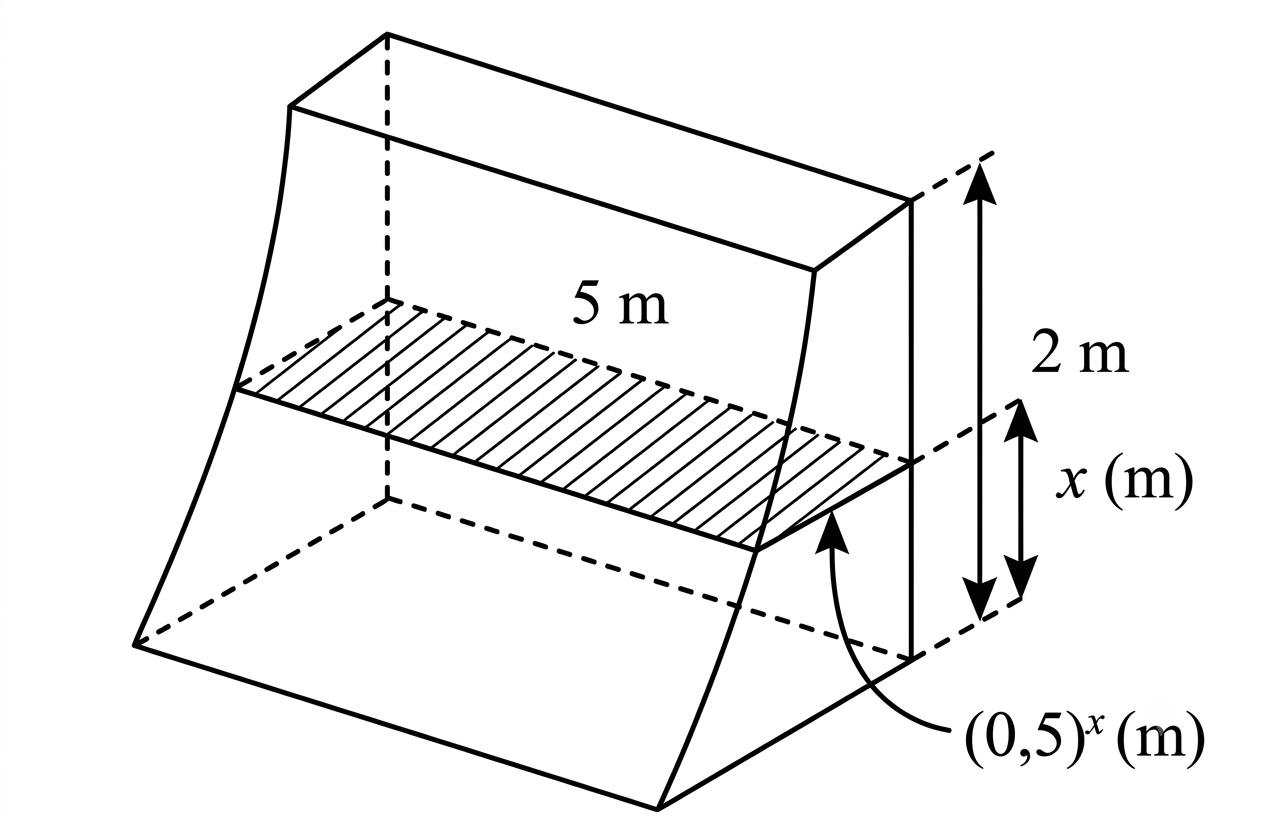
\includegraphics[width=0.4\textwidth]{images/V48.png}
\end{figure}

}

\questionShortAnswer{20}{49}{Bạn Hải nhận thiết kế logo hình con mắt (phần được tô đậm) cho một cơ sở y tế. Logo là hình phẳng giới hạn bởi hai parabol \( y = f(x) \) và \( y = g(x) \) như Hình (đơn vị trên mỗi trục toạ độ là decimét). Bạn Hải cần tính diện tích của logo để báo giá cho cơ sở y tế đó trước khi kí hợp đồng. Diện tích của logo là bao nhiêu decimét vuông (làm tròn kết quả đến hàng phần mười).

\begin{center}
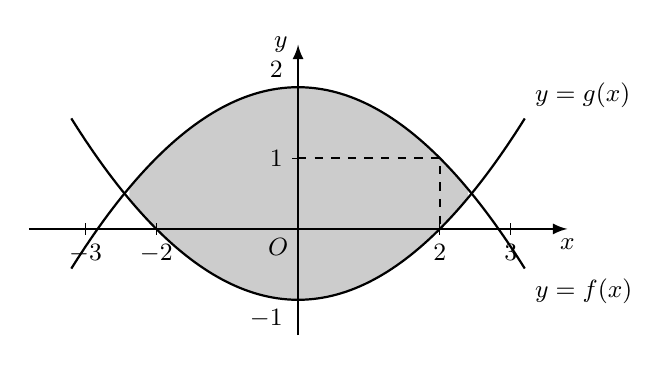
\begin{tikzpicture}[>=latex, scale=0.9]
    % 1. Tô màu xám miền giới hạn giữa hai parabol từ giao điểm x = -2.236 đến x = 2.236
    % Giao điểm của y = -0.25*x^2 + 2 và y = 0.25*x^2 - 1 là x = +-sqrt(6) ≈ +-2.45 (hoặc +-sqrt(5) ≈ +-2.236)
    \fill[gray!40] 
        plot[domain=-2.38:2.4, samples=100] (\x, {-0.25*\x*\x + 2}) -- 
        plot[domain=2.4:-2.38, samples=100] (\x, {0.25*\x*\x - 1}) -- cycle;

    % 2. Trục tọa độ
    \draw[->, thick] (-3.8,0) -- (3.8,0) node[below] {\small $x$};
    \draw[->, thick] (0,-1.5) -- (0,2.6) node[left] {\small $y$};
    \node[below left] at (0,0) {\small $O$};

    % 3. Đồ thị các hàm số
    % Parabol quay xuống y = f(x)
    \draw[thick, samples=100, domain=-3.2:3.2] 
        plot (\x, {-0.25*\x*\x + 2}) 
        node[below right] {\small $y = f(x)$};

    % Parabol quay lên y = g(x)
    \draw[thick, samples=100, domain=-3.2:3.2] 
        plot (\x, {0.25*\x*\x - 1}) 
        node[above right] {\small $y = g(x)$};

    % 4. Đường gióng nét đứt tại (2, 1)
    \draw[dashed, thick] (0,1) -- (2,1) -- (2,0);

    % 5. Đánh dấu các vạch và nhãn số trên các trục
    \draw (-3, 0.08) -- (-3, -0.08) node[below] {\small $-3$};
    \draw (-2, 0.08) -- (-2, -0.08) node[below] {\small $-2$};
    \draw (2, 0.08) -- (2, -0.08) node[below] {\small $2$};
    \draw (3, 0.08) -- (3, -0.08) node[below] {\small $3$};

    \draw (0.08, 2) -- (-0.08, 2) node[above left] {\small $2$};
    \draw (0.08, 1) -- (-0.08, 1) node[left] {\small $1$};
    \draw (0.08, -1) -- (-0.08, -1) node[below left] {\small $-1$};
\end{tikzpicture}
\end{center}
}

\questionShortAnswer{20}{50}{Cho hàm số \( y = x^2 - 2x \) có đồ thị \((C)\). Kí hiệu \( A \) là hình phẳng giới hạn bởi \((C)\), trục hoành và hai đường thẳng \( x = 0, x = 2; B \) là hình phẳng giới hạn bởi \((C)\), trục hoành và hai đường thẳng \( x = 2, x = a (a > 2) \). Tìm giá trị của \( a \) để \( A \) và \( B \) có diện tích bằng nhau.

\begin{center}
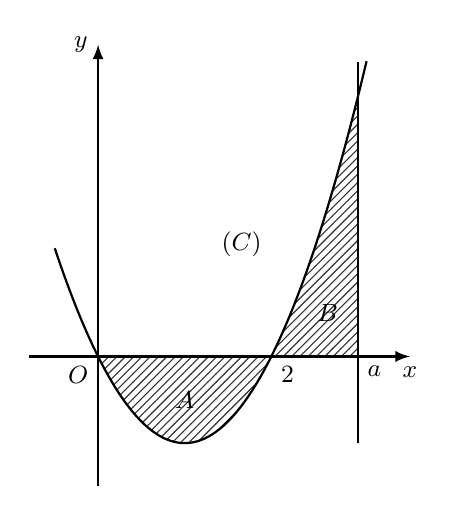
\begin{tikzpicture}[>=latex, scale=1.1]
    % Yêu cầu khai báo \usetikzlibrary{patterns} ở Preamble

    % 1. Tô gạch sọc đứng miền A (nằm dưới trục Ox từ 0 đến 2)
    % Hàm số bậc ba/bậc hai minh họa: y = x(x-2) = x^2 - 2x
    \fill[pattern=north east lines, pattern color=black!80] 
        plot[domain=0:2, samples=100] (\x, {\x*\x - 2*\x}) -- (0,0) -- cycle;

    % 2. Tô gạch sọc đứng miền B (nằm giữa đồ thị (C), trục Ox và đường x = a)
    % Với a = 3
    \fill[pattern=north east lines, pattern color=black!80] 
        (2,0) -- plot[domain=2:3, samples=100] (\x, {\x*\x - 2*\x}) -- (3,0) -- cycle;

    % 3. Trục tọa độ
    \draw[->, thick] (-0.8,0) -- (3.6,0) node[below] {\small $x$};
    \draw[->, thick] (0,-1.5) -- (0,3.6) node[left] {\small $y$};
    \node[below left] at (0,0) {\small $O$};

    % 4. Đồ thị đường cong (C)
    \draw[thick, samples=100, domain=-0.5:3.1] 
        plot (\x, {\x*\x - 2*\x});
    \node[left] at (2.0, 1.3) {\small $(C)$};

    % 5. Đường thẳng đứng x = a
    \draw[thick] (3, -1) -- (3, 3.4);

    % 6. Đánh dấu các nhãn điểm và miền
    \node[below right] at (2,0) {\small $2$};
    \node[below right] at (3,0) {\small $a$};

    \node at (1.0, -0.5) {\small $A$};
    \node at (2.65, 0.5) {\small $B$};
\end{tikzpicture}
\end{center}
}
\end{document}
